\documentclass{article}
\usepackage{graphicx}
\usepackage{amsmath}
\usepackage{amssymb}
\usepackage{natbib}
\usepackage{caption}
\usepackage{subcaption}
\usepackage{multicol}
\usepackage{color}
\usepackage{xspace}
\usepackage{enumerate}

%\bibliographystyle{elsarticle-num}


\begin{document}

\title{On a Geometric Forecast Method}

\author[1]{Babak Emami\corref{cor1}%
\fnref{fn1}}
\ead{babak.emami@gmail.com}
\cortext[cor1]{Corresponding author}
\fntext[fn1]{The author is an independent researcher.}
\address[1]{1335 Filbert St., 303, San Francisco, CA, United States 94109}

\begin{abstract}

A geometric method is porposed to forecast time series. Given a set of
correlated time series, it is assumed that the corresponding variables
follow a geodesic curve on a smooth real manifold. The corresponding
manifold connection is computed by assuming some constraints on the
form of connection. Once a conncetion is fixed, the future of the time
series can be computed by solving the geodesic equations subject to
appropriate boundary conditions. This yields a forecast of the time
series variables.

\end{abstract}

\maketitle

\section{Introduction}\label{section:introduction}

A framework to forecast multi-variable correlated time
series is proposed. The values of all variables at each time $t$
are assumed to be components of a vector tangent to a real
differentiable manifold $M$ at a point $p(t) \in M$. With this
assumption, the time series correspond to a set of vectors tangent to
$M$ at different points. These vectors form a path on $M$. Assuming
that this path is a geodesic on manifold $M$, one can infer some of
the structural properties of manifold $M$ from the data. This is then used to
forecast all variables, without depending on future values of any
predictors. Rather than taking a causal viewpoint by dividing
variables into responses and predictors, the proposed approach
searches for the logical relationship between variables by building
the above-mentioned manifold.

The present notes are an extension of the work discussed in
~\cite{emami-geo-2021}. There are two new aspects to what is discussed
here,

\begin{itemize}
    \item Rather than using a fixed boundary condition, the bounday
      condition values are now a subset of the model parameters. This
      is discussed in section~\ref{subsection:boundary-conditions}.
    \item Some of the new ideas that the author is working at present
      are discussed in section~\ref{section:future-work}.
\end{itemize}

The reader may refer to section 1 of \cite{emami-geo-2021} for a brief
discussion on the motivtion of current work as well as the literature
available on application of topology in data analysis and forecast
methods.

\section{Mathematical Framework}
\label{section:framework}

Let us assume that we are given $N$ observations $u^{m}(t_{i})$ over a
period of time $[0,T]$ for a set of $n$ correlated time dependent
variables $u^{m}$ where $m \in [1,n] \cap \mathbb{N}$, $i \in [1,N]
\cap \mathbb{N}$; $t_{i} \in [0,T]$ denotes the time of observation
$i$.

Let us now assume that observed values of these $n$ variables at time
$t_{i}$ are components of a vector $\mathbf{u}_{i}$ tangent to a
differentiable manifold $M$, with respect to the coordinate basis
$\{\partial_{m}|_{p_{i}}\}$ induced by a chart $(U, x)$, at a point
$p_{i} \in U \subseteq M$.

Without loss of generality, we can assume that the $N$ points $p_{i}$
lie on a smooth curve $\gamma:[0,T] \to M$, and that the $N$ vectors
$\mathbf{u}_{i} \in T_{p_{i}}M$ are tangent to this curve. Figure
\ref{fig:visualization} shows the coordinates $x^{1}$, $x^{2}$, and
$x^{3}$ of a curve corresponding to three arbitrary time dependent
variables $u^{1}$, $u^{2}$, and $u^{3}$. Here the vector tangent to
the curve at $p(t)$ is naively illustrated as an arrow. The components
of this vector are $u^{1}(t)$, $u^{2}(t)$, and $u^{3}(t)$.

\begin{figure}[h]
  \centering
  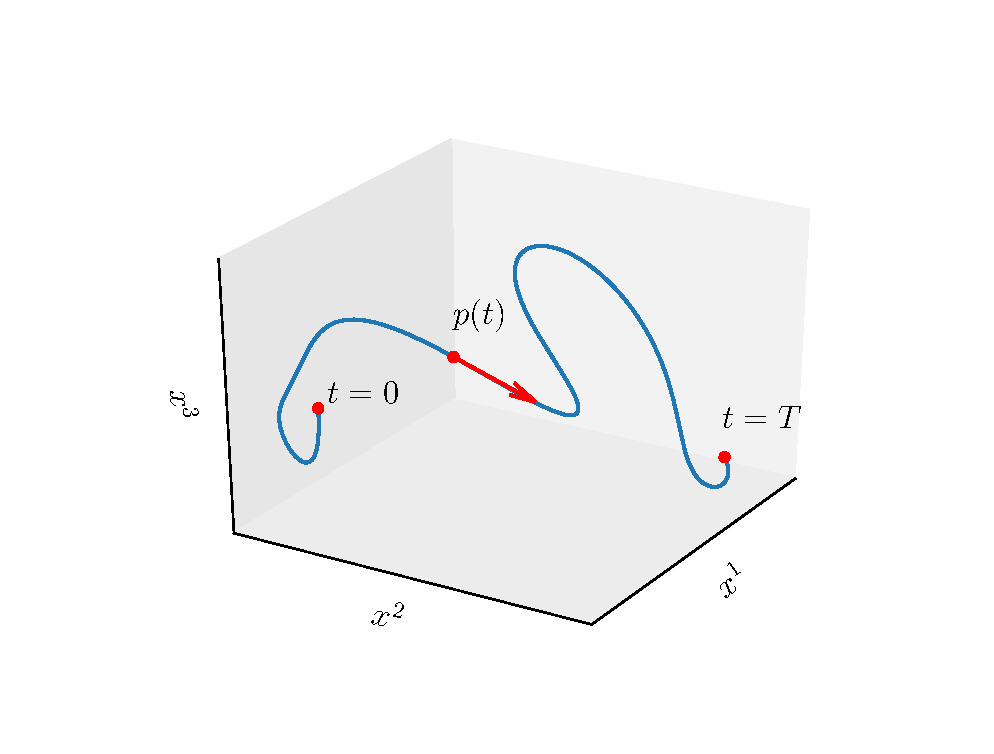
\includegraphics[scale=0.6, bb=0 0 461 346,trim={1cm 1cm 1cm 2cm},clip]{visualization.eps}
  \caption{Visualization of a smooth curve on a three dimensional
    manifold $M$ in coordinates $x^{1}$, $x^{2}$, and $x^{3}$
    corresponding to three time dependent variables $u^{1}$, $u^{2}$,
    and $u^{3}$. The values $u^{1}(t)$, $u^{2}(t)$, and $u^{3}(t)$ at
    time $t \in [0,T]$ are components of the vector tangent to this
    curve.}
  \label{fig:visualization}
\end{figure}

Let us now assume that this smooth curve is a
geodesic on $M$. The coordinates $x^{m}$ of the curve should then
satisfy the geodesic equations~\cite{deFelice-1990, schrodinger-1985},

\begin{equation}\label{eqn:geodesic-x}
\ddot{x}^{m} + \Gamma^{m}_{\;ab} \dot{x}^{a} \dot{x}^{b} = 0
\end{equation}

where $x^{m}(t)$ are coordinates of $p(t) \in M$, $\dot{x}^{m} =
\frac{dx^{m}}{dt}$, and $\Gamma^{m}_{\;ab} = \Gamma^{m}_{\;ab}(p(t))$
are Christoffel symbols. Note that the summation convention is in
effect. As $u^{m}$s are components of a tangent vector with respect to
basis $\{\frac{\partial}{\partial{x^{m}}}\}$ in $T_{p(t)}M$, we have
$u^{m}(t) = \frac{dx^{m} \circ p(t)}{dt}$, and so the geodesic
equations can be formulated in terms of $u^{m}$s,

\begin{equation}\label{eqn:geodesic}
\dot{u}^{m} + \Gamma^{m}_{\;ab} u^{a} u^{b} = 0
\end{equation}

Note that because connection is in fact a linear map $T_{p_1}M \to
T_{p_2}M$ that maps a vector tangent to $M$ at point $p_1$ to a vector
at point $p_2$, the above assumption implies that $u^{m}(t_{i})$ for a
fixed $m$ is a linear function of all $u^{r}(t_{i-1})$, that is
$u^{m}(t_{i}) = A^{m}_{r} u^{r}(t_{i-1})$, where summation convention
on $r$ is in effect.

We need to find a connection on manifold $M$, and thus its
corresponding Christoffel symbols in chart $(U,x)$, such that
equation~\ref{eqn:geodesic} holds. Once a connection is fixed,
equation~\ref{eqn:geodesic} subject to an appropriate boundary
condition can be solved to forecast $u^{m}(t)$ for $t \in (T,
\infty)$. The choice of connection is not unique. In fact, given that
information provided by $u^{m}(t)$ for $t \in [0,T]$ corresponds to
only one geodesic on $M$, the set of all connections that behave
similarly near the geodesic path are equally valid choices.

\subsection{Constraints on Connection}
\label{subsection:connection-constraints}

It may be useful to constrain the manifold connection by assuming
conditions on Christoffel symbols. Without any constraint, we need
$n^3 N$ parameters to represent $\Gamma^{m}_{\;ab}(p(t))$. Enforcing
constraints reduces the number of parameters and protects the model
against potential overfitting.

Here, we impose the following constraints,

\begin{itemize}
    \item The manifold is equipped with a
      Levi-Civita~\cite{deFelice-1990} connection, and thus a metric
      that is compatible with this connection. This indicates a
      symmetry in the lower indices of Christoffel symbols, that is
      $\Gamma^{m}_{\;ab} = \Gamma^{m}_{\;ba}$.
    \item Christoffel symbols associated with the connection with
      respect to the fixed chart $(U,x)$ are constant in the vicinity
      if the geodesic path. This is a sufficient, but not necessary,
      condition for the manifold to have a constant curvature in the
      vicinity if the geodesic path.
    \item The components of the metric tensor with respect to the
      fixed chart $(U,x)$, say $g_{ij}$ are diagonal. That is, $g_{ij}
      = 0$ for all $i \neq j$. This indicates that
      $\Gamma^{m}_{\;ab}|_{m \ne a \ne b} = 0$.
    \item 
\end{itemize}

Imposing the above constraints reduces the number of indpendent
Christoffel symbols to $n(2n-1)$.

\subsection{Boundary condition}
\label{subsection:boundary-conditions}

We need a boundary condition to solve the system of ODEs in
equation~\ref{eqn:geodesic}. In general, we can impose a condition at
any $t \in [0,T]$. Naturally, one may choose to impose a condition either
at $t = 0$ or $t = T$. Here on, we assume that a condition is imposed
at $t = T$, that is,

\begin{equation}\label{eqn:geodesic-bc}
u^{m}(t = T) = \xi^{m}
\end{equation}

where $\xi^{m}$ are $n$ model parameters to be computed along with the
indpendent components of Christoffel symbols. The model thus has a
total of $2n^2$ parameters.

\subsection{Computation of Christoffel symbols}
\label{subsection:computation}

Computation of the Christoffel symbols with the above constraints can
be formulated as a constraint optimization problem. We have,

\begin{equation}\label{eqn:optimization-problem}
\min_{(\Gamma^{m}_{\;ab}, xi^{m})}
J(u^{1},...,u^{n},\hat{u}^{1},...,\hat{u}^{n})
\end{equation}

The objective function $J$ is defined as,

\begin{equation}\label{eqn:optimization-objective-raw}
J := \frac{1}{2} \int_{0}^{T} dt \sum_{m=1}^{n} (u^{m}(t) -
\hat{u}^{m}(t))^2
\end{equation}

where $u^{m}(t)$ and $\hat{u}^{m}(t)$ represent predicted and actual
time series, respectively.

Note that the choice of an objective function is obviously not
unique. The above problem is constrained to the geodesic
equation~\ref{eqn:geodesic} with boundary condition
~\ref{eqn:geodesic-bc}.  \xi^{m}$.

We need to solve \ref{eqn:optimization-problem} using an optimization
method. Most optimization methods need the gradient of the objective
function with respect to the optimization variables, that is
$\frac{dJ}{d \Gamma^{m}_{\;ab}}$ sand $\frac{dJ}{d \xi^{m}}$. As the
number of optimization variables is potentially large, the numerical
computation of all gradients is expensive. Instead, we can use an
approach which is generally referred to as the continuous adjoint
optimization method~\cite{adjoint-giles}. Using the adjoint method
allows one to compute the gradient of the objective function,
constrained by a differential equation, with respect to the
optimization variables, by solving an extra differential equation only
once per optimization iteration.

One can show that,

\begin{equation}\label{eqn:objective-gradient-1}
\frac{d J}{d \tilde{\Gamma}^{\alpha}} = \int_{0}^{T} v_{m} \frac{d
  \Gamma^{m}_{\;ab}}{d \tilde{\Gamma}^{\alpha}} u^{a} u^{b} dt
\end{equation}

and

\begin{equation}\label{eqn:objective-gradient-1}
\frac{d J}{d \xi^{m}} = -v_{m}( t = T )
\end{equation}

where $\tilde{\Gamma}^{\alpha}$ with $\alpha \in [1,n(2n-1)] \cap
\mathbb{N}$ are the independent components of $\Gamma^{m}_{\;ab}$, and
$v_{m}$ are called the adjoint variables and are solutions of a linear
ODE,

\begin{equation}\label{eqn:adjoint-equation}
\dot{v}_{s} - 2 \Gamma^{m}_{\;as} u^{a} v_{m} = \frac{df}{du^{s}}
\end{equation}

subject to a boundary condition,

\begin{equation}\label{eqn:adjoint-bc}
v_{r}( t = 0 ) = 0.
\end{equation}

Note that as $u^{m}$s are components of a tangent vector, $v_{m}$s are
components of a cotangent vector and therefore $\boldsymbol{v}(t) \in
T^{*}_{p(t)}M$ with respect to the dual basis induced by chart $(U,
x)$. The reader may refer to ~\cite{emami-geo-2021} for a detailed
derivation of equation~\ref{eqn:adjoint-equation} and to
\cite{adjoint-giles} for a detailed exposition of adjoint methods.

\section{Further Development}\label{section:future-work}


\bibliography{references}

\end{document}

